\documentclass[onecolumn, conference]{IEEEtran}
\IEEEoverridecommandlockouts
% The preceding line is only needed to identify funding in the first footnote. If that is unneeded, please comment it out.
\usepackage{cite}
\usepackage{amsmath,amssymb,amsfonts}
\usepackage{algorithmic}
\usepackage{graphicx}
\usepackage{textcomp}
\usepackage{xcolor}
\usepackage{tabularx}
\usepackage{adjustbox}
\usepackage{hyperref}
\usepackage{doi}
\usepackage[a4paper, left=3cm, right=3cm, top=2cm, bottom=2cm]{geometry}

\usepackage{tikz}
\usetikzlibrary{shapes.geometric, arrows, positioning}
\tikzstyle{startstop} = [ellipse, minimum width=3cm, minimum height=1cm, text centered, draw=black]
\tikzstyle{process} = [rectangle, minimum width=3cm, minimum height=1cm, text centered, draw=black]
\tikzstyle{arrow} = [thick,->,>=stealth]

\def\BibTeX{{\rm B\kern-.05em{\sc i\kern-.025em b}\kern-.08em
T\kern-.1667em\lower.7ex\hbox{E}\kern-.125emX}}

\begin{document}

\bibliographystyle{IEEEtran}

\title{Assessing Language Model Performance in Biomedical Question-Answering: A Case Study Using the LangChain Framework on the CliCR Dataset}

\author{\IEEEauthorblockN{1\textsuperscript{st} Feras AlMannaa}
  \textit{ferasmhdaymanalmanna@stu.aydin.edu.tr}
  \IEEEauthorblockA{S.N. Y2213.140002}
  \and
  \IEEEauthorblockN{2\textsuperscript{nd} MHD Yassin AlMannaa}
  \textit{myassinmannaa@stu.aydin.edu.tr}
  \IEEEauthorblockA{S.N. Y2213.140023}
}

\maketitle

\begin{abstract}
  This study explores the development of an advanced biomedical question-answering (BQA) system using large language models (LLMs) on the CliCR dataset, leveraging the LangChain framework. LLMs such as GPT-3.5, GPT-4, and open models like LLAMA3 and Mistral have been integrated to enhance response accuracy for clinical queries. The methodology has involved comprehensive data preparation, prompt engineering, model adaptation using LangChain's API tools, and rigorous evaluation with metrics including precision, recall, F1-score, BLEU scores, and embedding-based average score.

  Results have shown that utilizing the full case context significantly outperformed vector store indexing methods. Notably, GPT-4 achieved an exact match (EM) score of 44.7\%, surpassing human experts' 35\%, and an embedding-based average (E-avg) score of 0.80, indicating high semantic relatedness. These findings underscore the potential of integrating state-of-the-art LLMs within frameworks like LangChain for advancing biomedical QA systems.

  The study has also highlighted that while fine-tuning LLMs on biomedical datasets can enhance domain-specific performance, it risks overfitting and loss of generalization. Therefore, prompt engineering and leveraging full context windows have emerged as more practical approaches. Evaluations of both closed-source and open-source models have provided valuable insights into their strengths and limitations, contributing to best practices for deploying LLMs in specialized domains like biomedicine.

  In conclusion, this research demonstrates the transformative potential of advanced LLMs in BQA systems, paving the way for future refinements to improve clinical decision-making and medical education.
\end{abstract}

\section{Introduction}
The rapid advancements in large language models (LLMs) such as GPT-3.5, GPT-4, and LLAMA have significantly transformed various fields, including natural language processing (NLP), artificial intelligence (AI), and healthcare. These models have shown remarkable capabilities in understanding and generating human language, making them highly valuable for biomedical applications. In the biomedical domain, LLMs have demonstrated immense potential in tasks such as biomedical question-answering (BQA), where they assist clinicians, researchers, and patients by providing accurate and timely information \cite{Hiesinger2023}

Biomedical QA systems play a crucial role in automating the answers to complex clinical questions posed by healthcare professionals, patients, or medical students. These systems facilitate clinical decision-making, support medical education, and aid research endeavors \cite{Jin2021}. Despite significant progress in NLP and the usage of both closed-source models like GPT-3.5/4 and open-source models like LLAMA-3, challenges remain that warrant further investigation \cite{Kalyan2021}.

Despite the impressive advancements in NLP and the success of LLMs in various tasks, specialized models and techniques are still needed to address the unique challenges of biomedical question-answering (BQA). The biomedical domain requires precise and reliable information retrieval to support clinical decision-making, medical education, and research.

One of the primary challenges in BQA is the ability to understand and reason over complex medical contexts, which often involve technical terminology, specialized knowledge, and intricate relationships between different medical entities. Existing language models may struggle to capture the nuances and intricacies of biomedical information, leading to inaccurate or incomplete answers. For instance, fine-tuning stability in biomedical NLP remains a significant challenge, especially in low-resource domains \cite{Tinn2021}.

Another challenge is managing the diversity and complexity of biomedical queries, ranging from straightforward factual questions to intricate reasoning tasks involving multiple clinical factors. Developing models that can effectively handle this range of queries while maintaining high accuracy and relevance is crucial for practical applications in the healthcare domain \cite{Tran2023}. Additionally, the availability of high-quality biomedical datasets for training and evaluation purposes is limited, posing challenges for developing and benchmarking robust and generalizable models \cite{Wang2023} \cite{Wang2023a}.

\subsection{Our Contribution}
To address the aforementioned challenges, the study explores several key contributions:

1. \textbf{Adoption of State-of-the-Art LLMs:} The adaptation of advanced language models, including GPT-3.5, GPT-4o, LLAMA3, Mistral, and Cohere's Aya, specifically for the task of biomedical question-answering has been investigated. By leveraging the latest advancements in LLMs and their improved capabilities for long-context understanding and semantic text generation, the aim is to enhance the performance of BQA systems \cite{Ozyurt2020} \cite{Chen2023}.

2. \textbf{Comprehensive Evaluation Across Multiple Models:} The study evaluates and compares the performance of both closed-source and open-source LLMs on the CliCR dataset \cite{Suster2018}, a domain-specific dataset designed for machine reading comprehension in the medical domain. This comprehensive evaluation provides insights into the strengths and limitations of different models, addressing the need for accurate and reliable BQA systems \cite{Soman2023} \cite{Gu2020}. A comprehensive QA framework has been built on top of the LangChain framework to streamline the process of integrating and evaluating different LLMs.

3. \textbf{Exploration of Prompt Engineering and Context Utilization:} The impact of prompt engineering techniques and the effective utilization of context information on the performance of LLMs in BQA tasks has been investigated. By crafting well-formulated prompts and leveraging the full context window of LLMs, the aim is to enhance the understanding and generation of accurate and relevant answers to biomedical queries \cite{Chen2023}.

4. \textbf{Fine-tuning and Domain Adaptation:} By adapting the models to the specific language and knowledge patterns found in biomedical data, more specialized and accurate BQA systems have been developed \cite{Jeong2020} \cite{Miolo2021}. Based on these insights, and to further improve the performance of LLMs in the biomedical domain, the feasibility of fine-tuning on biomedical datasets has been explored.

Through these contributions, the study aims to advance the state-of-the-art in biomedical question-answering by leveraging the latest advancements in LLMs, conducting comprehensive evaluations, optimizing prompt engineering and context utilization, and exploring fine-tuning and domain adaptation techniques.

\section{Literature Review}

Several studies have evaluated the performance of LLMs in various biomedical QA tasks. Duong and Solomon \cite{Duong2023} compared the performance of ChatGPT with human respondents on genetics questions, finding that while ChatGPT performed similarly to humans on memorization-type questions, it struggled with critical thinking questions. This indicates the need for further refinement in LLMs to enhance their critical reasoning capabilities.

In another study, Lee et al. \cite{Lee2023} developed a privacy-preserving LLM for automated data extraction from thyroid cancer pathology reports. Their findings showed that the LLM achieved high concordance rates with human reviewers, suggesting its potential in clinical data extraction tasks while maintaining patient privacy.

Schubert et al. \cite{Schubert2023} assessed the performance of LLMs on neurology board-style examinations. They found that newer versions of LLMs outperformed human averages, particularly in behavioral, cognitive, and psych-related questions. This highlights the evolving accuracy and reliability of LLMs in specialized medical fields.

Kumari et al. \cite{Kumari2023} conducted a comparative study of ChatGPT-3.5, Google Bard, and Microsoft Bing in solving hematology cases. Their results indicated that ChatGPT outperformed the other models, demonstrating its superior capability in handling complex medical queries.

\subsection{Challenges and Limitations}
Despite the promising results, LLMs face several challenges in biomedical QA. Koga \cite{Koga2023} explored the pitfalls of LLMs in pathology board examinations, identifying issues such as inconsistency and inaccuracy in responses. These findings emphasize the need for ongoing model refinement and human oversight to mitigate errors.

Reese et al. \cite{Reese2023} evaluated the limitations of GPT-4 in clinical diagnosis, noting that its performance deteriorated when prompts lacked detailed narrative context. This suggests that LLMs require comprehensive input to provide accurate diagnostic reasoning, underscoring the importance of context in medical QA.

Pal et al. \cite{Pal2023} highlighted the issue of bias amplification in LLMs, particularly in clinical phenotyping. Their study demonstrated that LLMs selectively underdiagnosed certain subpopulations, raising concerns about the equitable application of these models in healthcare settings.

\subsection{Innovative Applications}
LLMs have shown potential in innovative applications beyond traditional QA tasks. For instance, Buckley et al. \cite{Buckley2023} evaluated the GPT-4V model on challenging medical cases involving both text and images. Their results indicated that GPT-4V outperformed human respondents, suggesting that multimodal AI models could enhance medical diagnostic reasoning.

Titus \cite{Titus2023} demonstrated the use of ChatGPT in biostatistics, guiding analyses of NHANES data. This study highlighted the model's ability to simplify complex data analysis, making statistical methods more accessible to non-experts.

Holmes et al. \cite{Holmes2023a, Holmes2023b, Holmes2023c} assessed LLMs in radiation oncology physics, finding that ChatGPT-4 performed comparably to medical physicists. This suggests the potential for LLMs to serve as knowledgeable assistants in highly specialized medical fields.

\subsection{Datasets and Methodologies}
Understanding the current state of research and existing methodologies in the field of Biomedical QA is pivotal for the development of advanced systems. This involves reviewing key datasets and techniques used for evaluation.

Šuster and Daelemans \cite{Suster2018} introduced the CliCR dataset, designed for machine comprehension in the medical domain, constructed from clinical case reports obtained from BMJ Case Reports. The dataset comprises approximately 100,000 gap-filling queries, providing a valuable resource for studying machine comprehension in the medical domain.

Jin et al. \cite{Jin2021} provide a comprehensive survey of BQA approaches and challenges, categorizing them into classic, information retrieval, machine reading comprehension, knowledge base, and question entailment approaches. Despite significant advancements in BQA, systems remain underutilized in real-life settings due to challenges such as system immaturity and limited practical application.

Kalyan et al. \cite{Kalyan2021} provide a comprehensive survey of transformer-based biomedical pretrained language models (BPLMs), highlighting their significance in NLP within the biomedical domain. The paper discusses foundational concepts, pretraining methods, tasks, fine-tuning techniques, and specific embedding types for biomedical applications.

Wang et al. \cite{Wang2022} also contribute to the understanding of domain-specific datasets, emphasizing the importance of specialized data for improving the accuracy and relevance of biomedical QA systems.

\subsection{Privacy and Ethical Considerations}
The use of LLMs in biomedical contexts raises significant privacy and ethical concerns. Research by Lee et al. \cite{Lee2023} on privacy-preserving LLMs highlighted the importance of maintaining patient confidentiality while leveraging the power of these models for data extraction and medical question answering. Their work demonstrated that with proper anonymization techniques, LLMs could be effectively used in clinical settings without compromising patient privacy.

Chowdhury \cite{Chowdhury2023} highlighted the potential of LLMs to address routine patient queries post-surgery but emphasized the need for safety measures to mitigate potential risks. This underscores the necessity for robust ethical guidelines and protocols to ensure the safe and responsible deployment of LLMs in healthcare.

\subsection{Future Directions}

The integration of autonomous agents powered by large language models (LLMs) in simulated environments, as demonstrated in the Agent Hospital study, offers a novel approach to enhancing the learning and adaptability of medical agents within the biomedical domain \cite{Li2024}.

The work simulated hospital environments where autonomous agents can learn and practice medical procedures could significantly improve the capabilities of BQA systems. These environments allow agents to accumulate experience and refine their decision-making processes in a controlled, risk-free setting. Future research should explore the development and integration of such simulacra to provide continuous learning opportunities for medical agents. It showcases the potential of evolutionary learning approaches in training doctor agents. By allowing agents to evolve and improve their treatment strategies over time, these methods can lead to more robust and accurate BQA systems. Investigating the application of similar evolutionary learning techniques to BQA models could enhance their performance and adaptability.

\begin{table*}[ht]
  \centering
  \caption{Comparative Analysis of Previous Works}
  \begin{tabularx}{\textwidth}{|X|X|X|X|X|}
    \hline
    \textbf{Study}                                & \textbf{Objective}                                                  & \textbf{Model Used}            & \textbf{Key Findings}                                                                      & \textbf{Technical Depth}                                                                                            \\
    \hline
    Duong and Solomon (2023) \cite{Duong2023}     & Evaluate ChatGPT vs. human respondents on genetics questions        & ChatGPT                        & ChatGPT performed well on memorization but struggled with critical thinking questions      & Comparison with human performance, identification of strengths and weaknesses in critical reasoning                 \\
    \hline
    Lee et al. (2023) \cite{Lee2023}              & Develop privacy-preserving LLM for data extraction from pathology   & Custom LLM                     & High concordance rates with human reviewers, maintained patient privacy                    & Custom LLM development, focus on privacy-preserving techniques, application in clinical data extraction             \\
    \hline
    Schubert et al. (2023) \cite{Schubert2023}    & Assess LLMs on neurology board-style examinations                   & Various LLMs                   & Newer LLMs outperformed human averages, particularly in behavioral and cognitive questions & Evaluation across multiple LLMs, detailed analysis of performance in specific medical fields                        \\
    \hline
    Kumari et al. (2023) \cite{Kumari2023}        & Compare ChatGPT-3.5, Google Bard, and Microsoft Bing on hematology  & ChatGPT-3.5, Google Bard, Bing & ChatGPT outperformed other models in handling complex medical queries                      & Comparative analysis of multiple models, focus on handling complex medical cases                                    \\
    \hline
    Koga (2023) \cite{Koga2023}                   & Explore pitfalls of LLMs in pathology board examinations            & GPT-4                          & Identified issues like inconsistency and inaccuracy in responses                           & Identification of LLM limitations, emphasis on the need for model refinement and human oversight                    \\
    \hline
    Reese et al. (2023) \cite{Reese2023}          & Evaluate limitations of GPT-4 in clinical diagnosis                 & GPT-4                          & Performance dropped without detailed narrative context                                     & Analysis of context importance in clinical diagnosis, evaluation of model limitations                               \\
    \hline
    Pal et al. (2023) \cite{Pal2023}              & Study bias amplification in LLMs in clinical phenotyping            & Various LLMs                   & LLMs underdiagnosed certain subpopulations                                                 & Examination of bias in LLMs, impact on equitable healthcare applications                                            \\
    \hline
    Buckley et al. (2023) \cite{Buckley2023}      & Evaluate GPT-4V on text and image-based medical cases               & GPT-4V                         & GPT-4V outperformed humans in multimodal medical diagnostic reasoning                      & Integration of text and image data, multimodal evaluation, performance comparison with humans                       \\
    \hline
    Titus (2023) \cite{Titus2023}                 & Use ChatGPT in biostatistics for analyzing NHANES data              & ChatGPT                        & Simplified complex data analysis, made statistical methods accessible to non-experts       & Application in biostatistics, focus on accessibility and simplification of complex analyses                         \\
    \hline
    Holmes et al. (2023) \cite{Holmes2023a}       & Assess LLMs in radiation oncology physics                           & ChatGPT-4                      & ChatGPT-4 performed comparably to medical physicists                                       & Evaluation in a specialized medical field, comparison with professional performance                                 \\
    \hline
    Šuster and Daelemans (2018) \cite{Suster2018} & Introduce CliCR dataset for machine comprehension in medical domain & Custom dataset                 & Dataset comprises 100,000 gap-filling queries from clinical case reports                   & Creation of a domain-specific dataset, focus on machine comprehension in the medical field                          \\
    \hline
    Jin et al. (2021) \cite{Jin2021}              & Survey of BQA approaches and challenges                             & Various approaches             & Identified underutilization in real-life settings due to system immaturity                 & Comprehensive survey, categorization of BQA approaches, identification of practical challenges                      \\
    \hline
    Kalyan et al. (2021) \cite{Kalyan2021}        & Survey of transformer-based biomedical pretrained language models   & Various BPLMs                  & Highlighted significance of BPLMs in NLP for biomedical domain                             & Detailed survey of transformer-based models, discussion of pretraining methods, tasks, and fine-tuning techniques   \\
    \hline
    Wang et al. (2022) \cite{Wang2022}            & Understand domain-specific datasets for BQA                         & Various datasets               & Emphasized the importance of specialized data for improving accuracy and relevance         & Analysis of domain-specific datasets, focus on the impact of specialized data on BQA performance                    \\
    \hline
    Li et al. (2024) \cite{Li2024}                & Explore use of autonomous agents in simulated hospital environments & Autonomous agents, LLMs        & Agents learned and practiced medical procedures, improving decision-making processes       & Simulation of hospital environments for agent training, evolutionary learning approaches in medical decision-making \\
    \hline
  \end{tabularx}
\end{table*}

\section{Methodology, Materials and Methods}

\subsection{Methodology}
This research has leveraged state-of-the-art large language models (LLMs) and natural language processing algorithms and tools along with the LangChain framework to develop a sophisticated Biomedical Question Answering system. The study comprises three key stages: data preparation, model adaptation, and evaluation. (Figure \ref{fig:langchain_pipeline}) shows a detailed pipeline of the work, and the details of each step are as follows:

\begin{enumerate}
  \item \textbf{Data Preparation:} In the first phase, the Clinically Informed Reading Comprehension (CliCR) dataset has been processed to make it suitable for utilization by different large language models. Key steps involve:
        \begin{enumerate}
          \item \textit{Data transformation:} Data transformation tasks have been carried out, such as loading the dataset, transforming its structure, cleaning, vectorization, and many other text processing tasks like lemmatization and lowercasing. These tasks vary depending on the selected prompting strategy (more on this in the next step) and the model being adapted.

          \item \textit{Handling Long Passages:} The average length of passages (approximately 1,466 tokens) is suitable for most large language models context windows. Some of the cases exceed the maximum context window of many local LLMs, which means different strategies to divide the content into smaller, manageable chunks might need to be tested and implemented, possibly using a sliding window technique.

          \item \textit{Prompt engineering:} The dataset is designed in a way that imposes restrictions on the predicted answer format. In this step, the best prompt likely to result in the correct answer has been engineered. Different versions of the prompt have been tested to align it with the selected LLM's capabilities.
        \end{enumerate}

  \item \textbf{Model Adaptation with LangChain:} Since the advancement of local, open-source LLMs has skyrocketed in the past few months, both the famous Generative Pertained Transformer (GPT) model, which is a state-of-the-art closed large language model including its different versions, and the state of the art open source and local models like LLAMA3, Mistral, and Command-R have been employed to compare their performance. They have been adapted to the dataset by exploring multiple methods and prompts. To keep the work LLM agnostic, an open-source generative language framework called LangChain has been employed. LangChain assists in wrapping LLMs’ functionalities in an accessible manner, making it simpler to switch the underlying LLM, data storage, and transformation tools easily to apply the same work using different LLMs and storage engines.

  \item \textbf{Evaluation:} Post adaptation, the system’s performance has been evaluated using multiple evaluation methods, mainly, exact match (EM), F1 score, BLEU score (B-2 and B-4), and an embedding-based metric (E-avg) (Table \ref{tab:metrics}). The results have then been compared to the results reported in the main dataset paper and future work has been planned.
\end{enumerate}

\begin{figure*}[htbp]
  \centering
  \resizebox{\textwidth}{!}{%
    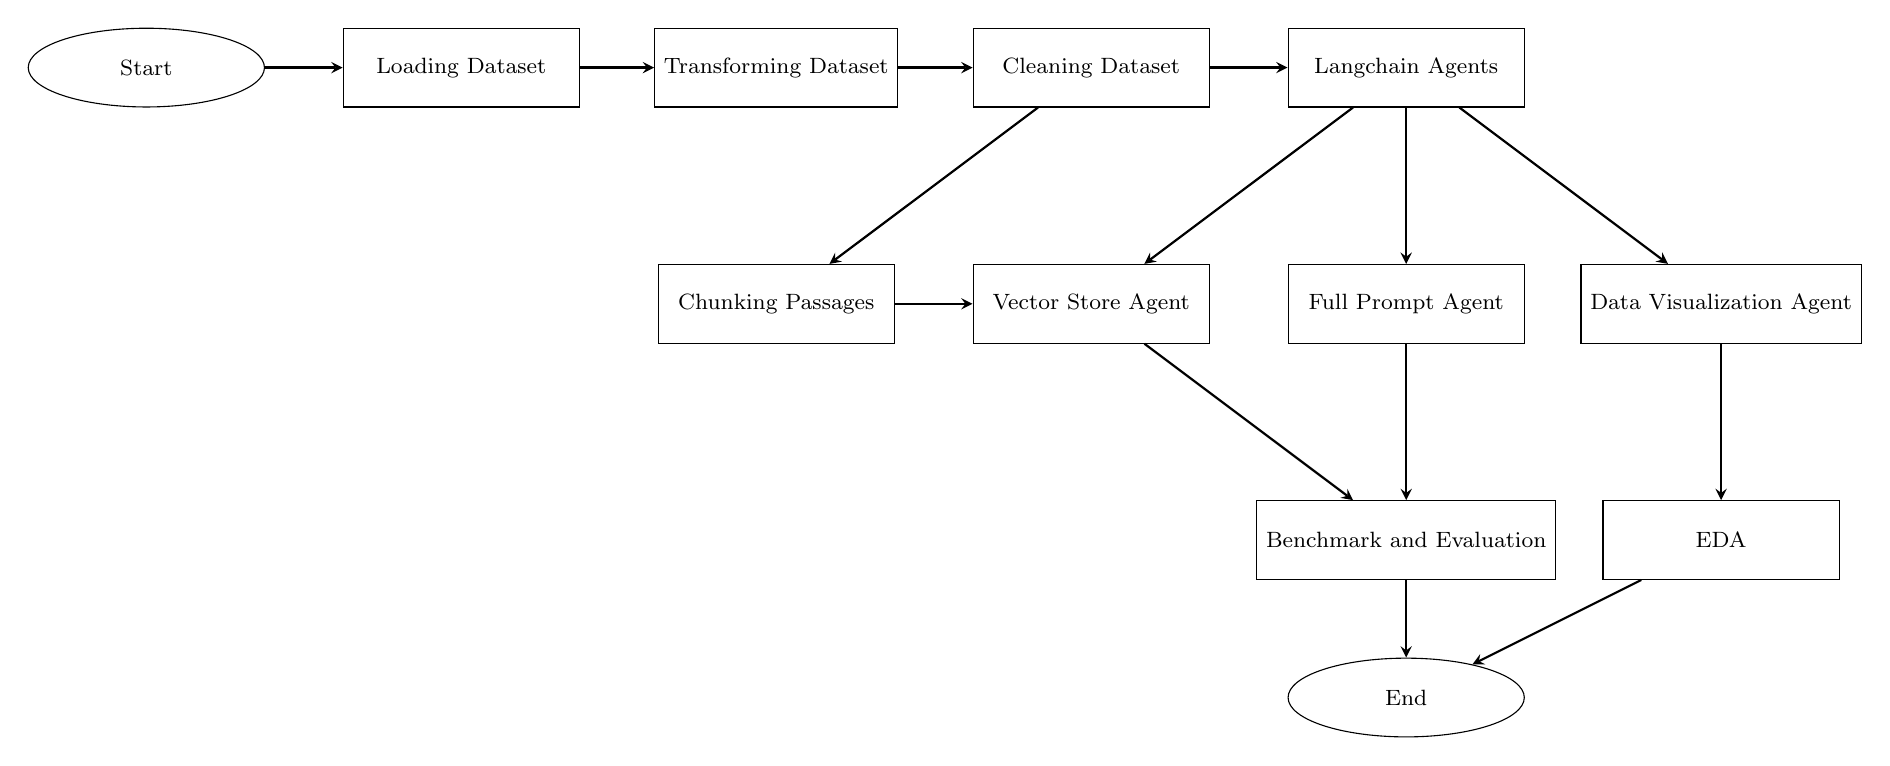
\begin{tikzpicture}[node distance=2cm, font=\footnotesize]

      % Nodes
      \node (start) [startstop] {Start};
      \node (load) [process, right of=start, xshift=2cm] {Loading Dataset};
      \node (transform) [process, right of=load, xshift=2cm] {Transforming Dataset};
      \node (clean) [process, right of=transform, xshift=2cm] {Cleaning Dataset};

      \node (chunk) [process, below of=transform, yshift=-1cm] {Chunking Passages};
      \node (proc) [process, right of=clean, xshift=2cm] {Langchain Agents};
      \node (viz) [process, below of=proc, yshift=-1cm, xshift=4cm] {Data Visualization Agent};
      \node (fc) [process, below of=proc, yshift=-1cm, xshift=0cm] {Full Prompt Agent};
      \node (vc) [process, below of=proc, yshift=-1cm, xshift=-4cm] {Vector Store Agent};

      \node (display) [process, below of=viz, yshift=-1cm] {EDA};
      \node (benchmark) [process, below of=fc, yshift=-1cm] {Benchmark and Evaluation};

      \node (end) [startstop, below of=proc, yshift=-6cm] {End};

      % Arrows
      \draw [arrow] (start) -- (load);
      \draw [arrow] (load) -- (transform);
      \draw [arrow] (transform) -- (clean);
      \draw [arrow] (clean) -- (proc);
      \draw [arrow] (clean) -- (chunk);
      \draw [arrow] (proc) -- (fc);
      \draw [arrow] (proc) -- (vc);
      \draw [arrow] (proc) -- (viz);
      \draw [arrow] (viz) -- (display);
      \draw [arrow] (chunk) -- (vc);
      \draw [arrow] (fc) -- (benchmark);
      \draw [arrow] (vc) -- (benchmark);
      \draw [arrow] (display) -- (end);
      \draw [arrow] (benchmark) -- (end);

    \end{tikzpicture}%
  }
  \caption{LangChain Agents Pipeline}
  \label{fig:langchain_pipeline}
\end{figure*}

\begin{table}[h]
  \centering
  \caption{Description of Evaluation Metrics}
  \begin{tabular}{|l|p{4cm}|p{6cm}|}
    \hline
    \textbf{Metric}               & \textbf{Description}                                                                                                                                                      & \textbf{Equation} \\
    \hline
    Exact Match (EM)              & Measures the percentage of instances where the predicted answer exactly matches the ground truth answer.                                                                  & \[
      \text{EM} = \frac{1}{N} \sum_{i=1}^{N} \text{I}(A_i = P_i)
    \]
    where \(A_i\) is the actual answer, \(P_i\) is the predicted answer, and \(\text{I}\) is the indicator function.                                                                                                              \\
    \hline
    F1 Score                      & Captures the overlap between the predicted and ground truth answers. It is the harmonic mean of precision and recall.                                                     & \[
      \text{F1} = 2 \cdot \frac{\text{Precision} \cdot \text{Recall}}{\text{Precision} + \text{Recall}}
    \]
    \[
      \text{Precision} = \frac{TP}{TP + FP}
    \]
    \[
      \text{Recall} = \frac{TP}{TP + FN}
    \]
    \(TP\) = True Positives, \(FP\) = False Positives, \(FN\) = False Negatives.                                                                                                                                                  \\
    \hline
    BLEU-2                        & Assesses token contiguity up to 2-grams. It is a popular metric for machine translation that measures the similarity between the predicted sequence and the ground truth. & \[
      \text{BLEU} = \text{BP} \cdot \exp \left( \sum_{n=1}^{2} w_n \log p_n \right)
    \]
    For BLEU-2, \(N=2\), where \(p_n\) is the precision of n-grams and \(w_n\) are the weights. \newline
    \[
      \text{BP} =
      \begin{cases}
        1                     & \text{if } c > r    \\
        e^{(1 - \frac{r}{c})} & \text{if } c \leq r
      \end{cases}
    \]
    \(c\) is the length of the candidate translation and \(r\) is the length of the reference translation.                                                                                                                        \\
    \hline
    BLEU-4                        & Similar to BLEU-2, but assesses token contiguity up to 4-grams.                                                                                                           & \[
      \text{BLEU} = \text{BP} \cdot \exp \left( \sum_{n=1}^{4} w_n \log p_n \right)
    \]
    For BLEU-4, \(N=4\). The brevity penalty \(BP\) is calculated as in BLEU-2.                                                                                                                                                   \\
    \hline
    Embedding-based (E-avg) Score & Measures semantic relatedness between the predicted and ground truth answers by comparing their vector embeddings.                                                        & \[
      \text{E-avg} = \frac{1}{N} \sum_{i=1}^{N} \cos(E_{A_i}, E_{P_i})
    \]
    where \(E_{A_i}\) is the embedding of the actual answer, \(E_{P_i}\) is the embedding of the predicted answer, and \(\cos\) is the cosine similarity.                                                                         \\
    \hline
  \end{tabular}
  \label{tab:metrics}
\end{table}

\subsection{Large Language Models}

Large language models (LLMs) have revolutionized the field of natural language processing (NLP) by demonstrating remarkable capabilities in understanding and generating human language. These models are typically based on transformer architectures, which enable them to process large amounts of text data and capture complex linguistic patterns. LLMs are pretrained on vast datasets and can be fine-tuned for specific tasks, making them highly versatile tools in various domains, including biomedical question-answering (BQA).

\begin{enumerate}
  \item \textbf{GPT (Generative Pre-trained Transformer):} The GPT series, developed by OpenAI, includes models like GPT-3.5 and GPT-4. These models are known for their impressive ability to generate coherent and contextually relevant text based on a given input prompt. GPT-3.5 and GPT-4 have been particularly successful in numerous NLP tasks, demonstrating high performance in text generation, translation, summarization, and question-answering tasks \cite{openai2024gpt4}. GPT-4, the latest in the series, has shown even greater improvements in language understanding and generation capabilities, making it a strong candidate for BQA systems.

  \item \textbf{LLAMA3:} LLAMA3, developed by Meta AI (formerly Facebook AI), is an open-source language model designed to provide high performance while being accessible to researchers and developers. LLAMA3 builds on the strengths of its predecessors and incorporates improvements in training techniques and architecture. This model aims to offer competitive performance in various NLP tasks, including biomedical question-answering, while maintaining an open-source philosophy \cite{touvron2023llama}.

  \item \textbf{Mistral:} Mistral is another open-source language model that emphasizes efficient training and inference. Developed to handle complex language tasks with fewer computational resources, Mistral leverages advancements in model compression and quantization. This makes it suitable for deployment in resource-constrained environments without compromising on performance. Mistral's capabilities in understanding and generating text make it a viable option for BQA systems \cite{jiang2023mistral}.

  \item \textbf{Cohere's Aya:} Cohere's Aya is an advanced language model developed by Cohere. Aya is designed to excel in generating high-quality, contextually relevant text across various domains. Cohere has focused on creating a model that balances performance and accessibility, making Aya a strong contender for tasks like biomedical question-answering. Aya's ability to integrate contextual information and generate accurate responses is particularly beneficial for BQA applications \cite{cohere2023aya}.
\end{enumerate}

The integration of these state-of-the-art LLMs within frameworks like LangChain enables the development of sophisticated BQA systems capable of providing accurate and reliable information for clinical queries.

The following models' weights have been chosen to evaluate:
\begin{itemize}
  \item Closed -  GPT-3.5
  \item Closed -  GPT-4o
  \item Open -    LLAMA3 7B
  \item Open -    Mistral 7B
  \item Open -    Cohere's Aya 8B
\end{itemize}

All open models have been evaluated using 4-bit quantization and were running locally on a Geforce 3070ti GPU. The closed models were evaluated using their respective APIs.

\subsection{CliCR: A Dataset of Clinical Case Reports for Machine Reading Comprehension \cite{Suster2018}}
The dataset used in this paper is domain-specific \cite{Wang2022} and is designed for machine comprehension in the medical domain and is constructed from clinical case reports obtained from BMJ Case Reports, the largest online repository of such documents. The dataset comprises approximately 100,000 gap-filling queries.

The clinical case reports in this dataset provide detailed descriptions of individual patient cases, focusing on rare diseases, unusual presentations of common conditions, and novel treatment methods. Each case report contains a section called "Learning points," which summarizes the key information from the report.

To construct the queries, the authors blank out a medical entity from one of the learning points in each case report. These learning points are paraphrased portions of the passage text and may not match the exact sentences in the passage. The missing entity becomes the target answer for the query.

To ensure the quality of the dataset, the authors perform several checks and refinements. The case reports are processed to remove HTML boilerplate and are tokenized using the cTakes toolkit. An entity recognition tool called Clamp is then applied to annotate the medical entities in the reports, providing concept unique identifiers (CUIs) that link the entities to the UMLS Metathesaurus.

The dataset statistics show that it contains around 11,846 cases, with a total of approximately 16.5 million tokens in the support passages. There are a variety of medical entity types in the passages, with a total of 591,960 distinct entity types. The dataset includes around 56,000 distinct answers, most of which are multi-word medical entities.

In terms of medical specialties, the dataset covers a wide range, with the most common specialties being radiology, gastrointestinal surgery, emergency medicine, respiratory medicine, and video reports.

The dataset provides a valuable resource for studying machine comprehension in the medical domain, allowing researchers to analyze the performance of different models and explore the comprehension skills required to answer questions accurately.

\subsection{Data Analysis}
Exploratory Data Analysis (EDA) plays a crucial role in this research as it provides a comprehensive understanding of the dataset and informs the structure of the Question-Answering (Q/A) system. By conducting EDA, insights into how the data is organized, its distribution, and key patterns have been gained.

Understanding how the data looks is vital for designing an effective Q/A system. EDA allows exploration of the dataset's characteristics, such as the types of clinical queries and the corresponding expert answers. By analyzing the distribution of the data, the frequency of certain query types, answer lengths, and variations can be identified. This information guides the structuring of the Q/A system to handle different query formats and optimize the retrieval of relevant passages.

The insights derived from EDA directly impact the main components of the system, namely prompt engineering and case context retrieval. Prompt engineering involves crafting well-formulated questions or prompts that yield accurate answers. Through EDA, an understanding of the variations and nuances in the queries is gained, enabling the development of prompt engineering strategies that account for these complexities.

Additionally, EDA helps assess the correlation between the queries and the cases. By analyzing the relationships between the queries and their corresponding passages, the most effective tools or techniques to use for passage retrieval can be determined. For example, if there is a strong correlation between certain keywords in the queries and the relevant passages, these keywords can be prioritized in the retrieval process.

In summary, EDA serves as the foundation for understanding the dataset and structuring the Q/A system. It allows exploration of the data's distribution, assessment of the correlation between queries and cases, and optimization of the components of prompt engineering and case context retrieval. By leveraging the insights from EDA, a more robust and accurate Q/A system for retrieving relevant passages in response to clinical queries can be designed.

\subsection{An Exhaustive Look at the CliCR Dataset}

Before diving into the implementation, it's crucial to understand the raw corpus that will form the bedrock of the work - the CliCR dataset. Ideated and curated for the purpose of facilitating machine reading in the medical domain, this dataset is derived from a compilation of nearly 12,000 case reports. These cases have been extracted from the reputable medical journal, 'BMJ Case Reports', and constitute a decade’s worth of data spanning from 2005 to 2016. The dataset is unique in its makeup - the case reports have been processed to generate approximately 100,000 queries. This resulted from masking or obscuring a specific medical entity within the learning points section of each report, thereby yielding queries that are closely tied to the supporting passages.

The CliCR dataset boasts an extensive and rich linguistic corpus, with an average passage length of about 1,500 tokens. Medical entity answers in the dataset can span from a single word to a collection of words. The statistical breakdown of the dataset can be seen in Table \ref{tab:data_statistics}.

\begin{table}[ht]
  \centering
  \caption{Statistical overview of the CliCR dataset. For token count in passages, each passage is counted only once, even though multiple queries may be associated with a single passage. \cite{Suster2018}}
  \label{tab:data_statistics}
  \begin{tabular}{l r}
    \textbf{Data Statistics}                         &             \\
    \hline
    Number of cases                                  & 11,846      \\
    Number of queries                                & 104,919     \\
    Total token count in passages without recounting & 16,544,217  \\
    Total token count in passages with recounting    & 153,784,539 \\
    Average length of passages (tokens)              & 1,465.75    \\
    Number of unique word types in passages          & 112,673     \\
    Number of unique entity types in passages        & 591,960     \\
    Queries in the training set                      & 91,344      \\
    Queries in the development set                   & 6,391       \\
    Queries in the test set                          & 7,184       \\
    Answer type: problem                             & \%71.92     \\
    Answer type: treatment                           & \%17.64     \\
    Answer type: test                                & \%10.43     \\
  \end{tabular}
\end{table}

Given the goal of this study, the CliCR dataset presents an invaluable opportunity to test the efficacy of both closed and open large language models in the biomedical domain. While the sheer volume of data and the complexity of the queries pose a formidable challenge, they also offer immense potential for training more sophisticated models and proving their effectiveness in the medical domain.

However, it's important to be mindful of the limitations posed by larger language models, especially with regard to the context window both in terms of reaching a hard limit of the maximum content windows of an LLM, and with the relative performance as the context window grows. Since its length restricts the amount of information the model can process simultaneously or affects its performance, an alternative strategy would be to employ vector space database systems to store and query pertinent information and incorporate them into the context in a phased manner. This step can help tackle context window limitations and improve model performance.

A two-step approach to enhance the performance of an open-source large language model for complex medical queries has been proposed. First, 'fine-tuning' the model using the CliCR dataset has been suggested. This process, while computationally demanding, is designed to improve the model's accuracy. Second, a thorough exploration of the CliCR dataset has been recommended. By understanding the dataset in depth, better application to the model can be achieved. These steps, although resource-intensive, are crucial for optimizing the use of LLMs for the specific task.

By developing a versatile model capable of dealing with unique challenges in medical question answering, it is believed that this work could contribute significantly towards advancing NLP applications in the biomedical domain.

\subsection{Data Exploration}

Conducting an extensive exploration of the CliCR dataset is an integral part of this research. Inspecting the dataset using a variety of visualization and statistical techniques has enabled the unmasking of its complexities and inherent characteristics. These insights have been utilized to maximize the accuracy of the model and mitigate potential setbacks, ensuring optimal performance.

Exploration started by consolidating fundamental statistical attributes about the dataset, which are encompassed in Table \ref{tab:data_statistics}. This table exhibits an overview of the data, including values such as the total number of cases (11,846) and tokens in the passages (16,544,217 without recounting and 153,784,539 with recounting), facilitating an initial comprehension of the dataset's structure.

The distribution of answer lengths depicted in Figure \ref{fig:passage_length} (a) stands out as a remarkable discovery. It suggests that most answers range from 1 to 5 words in length, the majority being of length 2. However, longer answers, extending beyond 20 words, are also present, albeit less frequently. This range of answer lengths implicates the need for a flexible model capable of handling answers spanning various lengths effectively.

Turning attention to the nature of answers within the dataset, it has been unearthed that numerous expressions could signify the same answer concept. Evidenced by the presence of 56,093 distinct answers, which balloon up to 288,211 when considering extended answers, which account for variances in phrasing or interpretation. This led to the comprehension of the importance of creating a model that can not only understand different answers but can also generalize across different ways of framing the same answer.

Contrasting this, an exploration into the most frequent answers in the dataset revealed that terms such as "treatment," "symptoms," "surgery," and "MRI" were recurrently witnessed (Table \ref{fig:answer_type_stats}). These terms provide a glimpse into the common subject matters addressed in the case reports, thereby serving as key indicators for the type of medical knowledge that the model must acquire and apply.

\begin{figure}
  \centering
  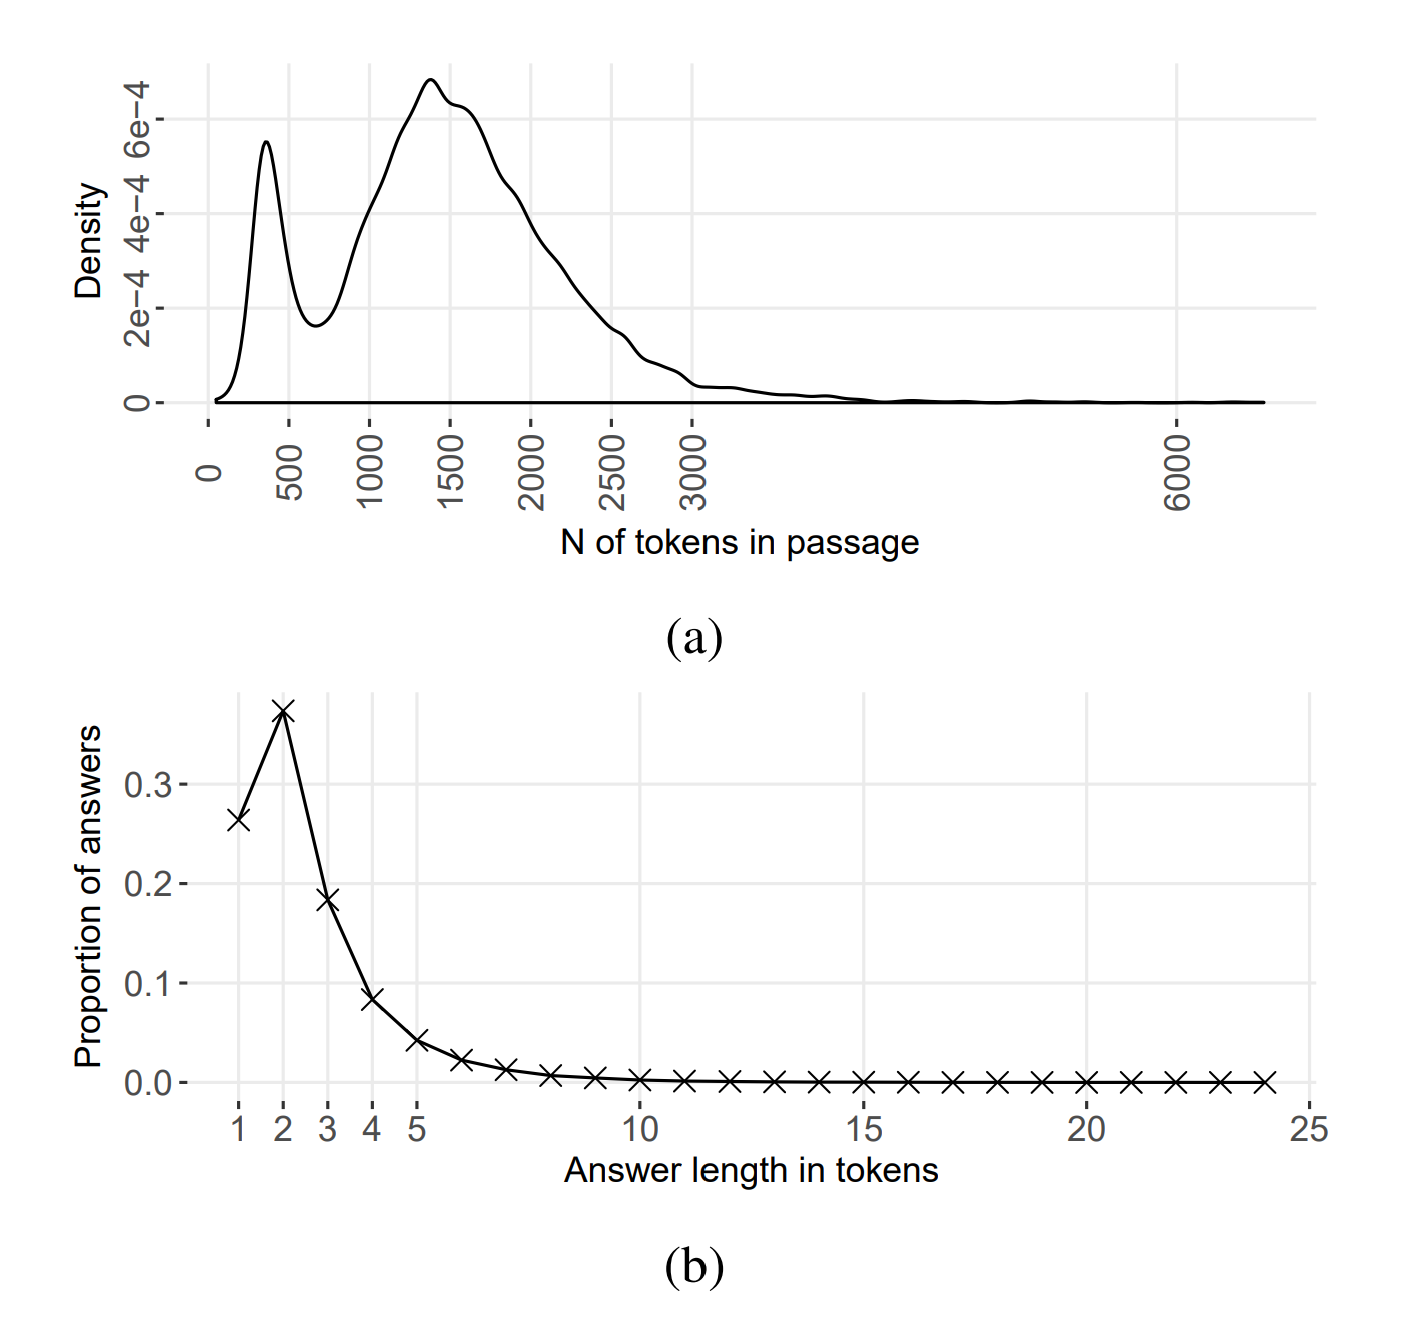
\includegraphics[width=\linewidth]{1.png}
  \caption{Distribution of answer lengths in the CliCR dataset. \cite{Suster2018}}
  \label{fig:passage_length}
\end{figure}

\begin{figure}
  \centering
  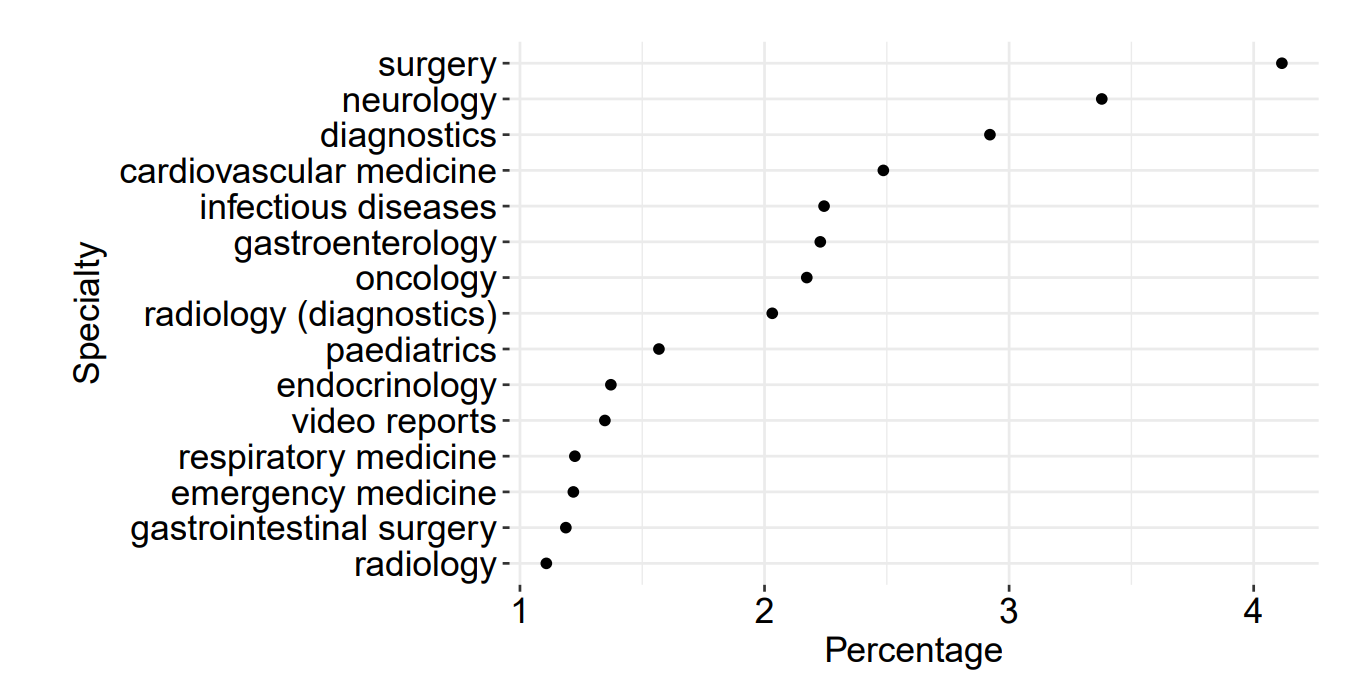
\includegraphics[width=\linewidth]{2.png}
  \caption{15 most common medical specialties. \cite{Suster2018}}
  \label{fig:answer_type_stats}
\end{figure}

The presence of the correct answers within the passages was another notable finding. About 58.94\% of answers were nestled directly within the corresponding passages. This demonstrates that in a significant number of instances, the model needs to decipher the context to formulate an appropriate response. This realization has been critical in informing the choice of architectural components of the model, emphasizing context-understanding mechanisms such as a transformer-based model.

Finally, through exploration, it has been observed that an increased presence of data answers (88.67\%) was seen when considering any passage in the dataset. This indicates that beyond mere retrieval of existing information, the model must be equipped to generate novel responses, adding another layer of complexity to the task of formulating a capable language model.

In summary, the exploration of the CliCR dataset has equipped valuable insights into the complexities and nuances of the data being dealt with. These findings serve as a guide in the subsequent steps of the study, aiding in formulating effective strategies for preprocessing, modeling, and evaluation phases, among others.

\section{Results}

\begin{table}
  \caption{GPT3.5 full case/vector retrieval}
  \centering
  \begin{tabular}{|c|c|c|c|c|c|} \hline
    \textbf{Method}     & \textbf{EM} & \textbf{F1} & \textbf{BLEU-2} & \textbf{BLEU-4} & \textbf{E-avg} \\ \hline
    GPT-3.5 - Full Case & 36.9\%      & 53.1\%      & 0.35            & 0.17            & 0.76           \\ \hline
    GPT-3.5 - Retrieval & 23.9\%      & 36.9\%      & 0.19            & 0.07            & 0.68           \\ \hline
  \end{tabular}
  \label{tab:fc_vec}
\end{table}

In this section, the results of the evaluation using multiple methods to improve the performance of the Question-Answering (Q/A) system are presented. The evaluation focused on prompt engineering, incorporating the large model, vector store indexing, and exploring the potential of fine-tuning.

Multiple LLMs have been chosen to include in this evaluation, both open and closed source, to compare their performance and measure the time and cost associated with each. These metrics help understand the capabilities and limits of each model and determine the most efficient and effective approach for the specific use case.

Additionally, the testing dataset has been minimized to reduce inference time and cost. By sampling a single question per case, representative results have been obtained while optimizing computational resources. This selection process strikes a balance between efficiency and evaluation accuracy.

First, the performance of running the same LLM using a full case in prompt and comparing it with running it using vector store indexing has been compared. The results are shown in Table \ref{tab:fc_vec}. The full case approach outperforms the vector store indexing approach in all metrics. This leads to the belief that the full case approach is more efficient and effective for the specific use case. At the same time, LLMs' context window limitations are not affecting the use case because the average length of the passages is suitable for most LLMs' context windows.

Secondly, the vector store indexing approach effectively retrieved relevant chunks of case context based on semantic similarity. By splitting the dataset into smaller chunks and indexing them, the most relevant chunks for each query have been retrieved. This approach performed worse than full prompt engineering, showcasing its weaknesses as an alternative method in the use case.

Table \ref{tab:evaluation} displays the evaluation results of each method for all LLMs. By crafting well-formulated prompts that included the complete case context, a significant improvement in the system's ability to generate accurate answers has been observed. The advancements in context window provided by all of the latest LLMs enhanced understanding and produced more comprehensive responses.

To assess performance, evaluation scores (Table \ref{tab:metrics}) including Exact Match (EM), F1 score, BLEU-2, BLEU-4, and embedding-based (E-avg) score have been utilized. The EM score measured the percentage of instances with exact matches between predicted and ground truth answers. The F1 score captured the overlap between predicted and ground truth answers. BLEU-2 and BLEU-4 assessed token contiguity, while the E-avg score measured semantic relatedness.

\begin{table}
  \centering
  \caption{Evaluation Results}
  \begin{tabular}{|c|c|c|c|c|c|c|} \hline
    \textbf{Method} & \textbf{EM}     & \textbf{F1}     & \textbf{BLEU-2} & \textbf{BLEU-4} & \textbf{E-avg} & \textbf{\%}      \\ \hline
    \multicolumn{7}{|c|}{Human baseline \cite{Suster2018}}                                                                      \\ \hline
    Human Expert    & 35\%            & 53.7\%          & \textbf{0.46}   & 0.23            & 0.67           & 100\%            \\ \hline
    Human Novice    & 31\%            & 45.1\%          & 0.43            & 0.24            & 0.62           & 92.5\%           \\ \hline
    \multicolumn{7}{|c|}{Previous Work \cite{Suster2018}}                                                                       \\ \hline
    rand-entity     & 1.4\%           & 5.1\%           & 0.03            & 0.01            & 0.23           & 34.3\%           \\ \hline
    maxfreq-entity  & 8.5\%           & 12.6\%          & 0.10            & 0.05            & 0.31           & 46.2\%           \\ \hline
    sim-entity      & 20.8\%          & 29.4\%          & 0.22            & 0.15            & 0.45           & 67.1\%           \\ \hline
    lang-model      & 2.1\%           & 3.5\%           & 0.00            & 0.00            & 0.30           & 44.7\%           \\ \hline
    SA-Anonym       & 19.6\%          & 27.2\%          & 0.22            & 0.16            & 0.43           & 64.1\%           \\ \hline
    SA-Ent          & 6.1\%           & 11.4\%          & 0.07            & 0.05            & 0.31           & 46.2\%           \\ \hline
    GA-Anonym       & 24.5\%          & 33.2\%          & 0.28            & 0.20            & 0.48           & 71.6\%           \\ \hline
    GA-Ent          & 22.2\%          & 30.2\%          & 0.25            & 0.18            & 0.46           & 68.6\%           \\ \hline
    GA-NoEnt        & 14.9\%          & 33.9\%          & 0.21            & 0.11            & 0.51           & 76.1\%           \\ \hline
    \multicolumn{7}{|c|}{Our Work}                                                                                              \\ \hline
    GPT-4o          & \textbf{44.7\%} & \textbf{60.9\%} & 0.43            & \textbf{0.24}   & \textbf{0.80}  & \textbf{119.4\%} \\ \hline
    GPT-3.5         & 36.9\%          & 53.1\%          & 0.35            & 0.17            & 0.76           & 113.4\%          \\ \hline
    AYA             & 34.3\%          & 50.6\%          & 0.42            & 0.27            & 0.70           & 104.4\%          \\ \hline
    Mistral         & 20.8\%          & 35.0\%          & 0.22            & 0.11            & 0.64           & 95.5\%           \\ \hline
    LLAMA3          & 17.1\%          & 31.3\%          & 0.12            & 0.05            & 0.61           & 91\%             \\ \hline
  \end{tabular}
  \label{tab:evaluation}
\end{table}

\section{Conclusion}

As per the results, the latest and most advanced LLM GPT-4o has outperformed all other models, including the human expert, which is a breakthrough in Q/A systems achievements. This indicates that the latest advancements in LLMs have a significant impact on the performance of Q/A systems. The results also show that lightweight open source models are gaining impressive understanding capabilities, what can be run today on consumer hardware is comparable to the top closed LLMs that were released a few months ago.

Unlike earlier studies that evaluated a limited set of models, this study has comprehensively assessed both closed (GPT-3.5, GPT-4o) and open (LLAMA3, Mistral, Cohere's Aya) LLMs using the CliCR dataset. This diverse evaluation provides a more complete understanding of LLM capabilities in BQA and addresses privacy and ethical considerations by offering evaluations for open, locally deployable LLMs.

Additionally, the performance of LLMs has been compared with human experts and novices, showing that GPT-4o outperforms human experts in exact match scoring, highlighting the rapid advancements in LLM capabilities.

In summary, prompt engineering and leveraging LLMs' full context window have yielded significant improvements in the Q/A system's performance compared to older NLP methods. Fine-tuning has proved less beneficial. Minimizing the testing dataset through strategic sampling reduced inference time and cost without compromising evaluation validity. Evaluation scores have provided a comprehensive understanding of precision, recall, token contiguity, and semantic relatedness. These findings contribute to more efficient and cost-effective approaches for enhancing Q/A systems within the medical domain.

\section{Future Work}

One area of future exploration is the evaluation of fine-tuning techniques. Although the initial evaluation did not yield substantial benefits from utilizing fine-tuned models, they might risk losing many of their general skills while getting too over-fitted on the dataset they were fine-tuned on, so further investigation is warranted. Therefore, conducting a comprehensive evaluation of fine-tuning methods and strategies would provide valuable insights into its effectiveness for the Q/A system.

In addition, the findings from the Agent Hospital study \cite{Li2024} present valuable insights and potential pathways for advancing BQA systems. By incorporating simulated training environments, evolutionary learning methods, and comprehensive knowledge integration, future BQA systems can achieve greater accuracy and effectiveness in supporting clinical decision-making and medical education.

In conclusion, future research should focus on incorporating extensive medical knowledge bases and leveraging LLMs to simulate complex medical scenarios, thereby improving the accuracy and reliability of the answers provided by BQA systems.

\bibliography{references}

\end{document}
